\documentclass[11pt]{article}
%\usepackage[14pt]{extsizes} % для того чтобы задать нестандартный 14-ый размер шрифта
%\usepackage[utf8]{inputenc}
\usepackage{mathtext}
\usepackage[english, russian]{babel}
\usepackage{amsmath}
\usepackage{amsfonts}
\usepackage{float}
\usepackage[margin=0.8in]{geometry}
\usepackage{multirow}
\usepackage{graphicx}
\usepackage[utf8x]{inputenc} % указать кодировку русского текста
\usepackage{fancyhdr}
\usepackage{indentfirst} % отступ в первой строке абзаца
\usepackage{wrapfig}
\usepackage{placeins}
\usepackage{wrapfig}
\usepackage{caption}
\usepackage{amssymb}
\usepackage{mathtools}
\usepackage[thinc]{esdiff}
\usepackage{cmap}
\usepackage[table,xcdraw]{xcolor}

\pagestyle{fancy}
\begin{document}
\begin{titlepage}
\begin{center}
%\vspace*{1cm}
\large{\small ФЕДЕРАЛЬНОЕ ГОСУДАРСТВЕННОЕ АВТОНОМНОЕ ОБРАЗОВАТЕЛЬНОЕ\\ УЧРЕЖДЕНИЕ ВЫСШЕГО ОБРАЗОВАНИЯ\\ МОСКОВСКИЙ ФИЗИКО-ТЕХНИЧЕСКИЙ ИНСТИТУТ\\ (НАЦИОНАЛЬНЫЙ ИССЛЕДОВАТЕЛЬСКИЙ УНИВЕРСИТЕТ)\\ ФИЗТЕХ-ШКОЛА РАДИОТЕХНИКИ И КОМПЬЮТЕРНЫХ ТЕХНОЛОГИЙ}
\vfill
\line(1,0){430}\\[1mm]
\huge{Лабораторная работа 3.1.1}\\
\huge\textbf{Магнитометр}\\
\line(1,0){430}\\[1mm]
\vfill
\begin{flushright}
\normalsize{Устюжанина Мария}\\
\normalsize{\textbf{Группа Б01-107}}\\
\end{flushright}
\end{center}
\end{titlepage}
\fancyhead[L] {Работа 3.1.1}

\par \textbf{Цель работы:} определить горизонтальную составляющую магнитного поля Земли и установить количественное соотношение между
единицами электрического тока в системах СИ и СГС.

\par \textbf{В работе используются:} магнитометр, осветитель со шкалой, источ­ник питания, вольтметр, электромагнитный переключатель, конденсатор, намагниченный стержень, прибор для определения периода крутильных колебаний, секундомер, рулетка, штангенциркуль.

\section{Экспериментальная установка}

\begin{wrapfigure}{r}{6.5cm}
    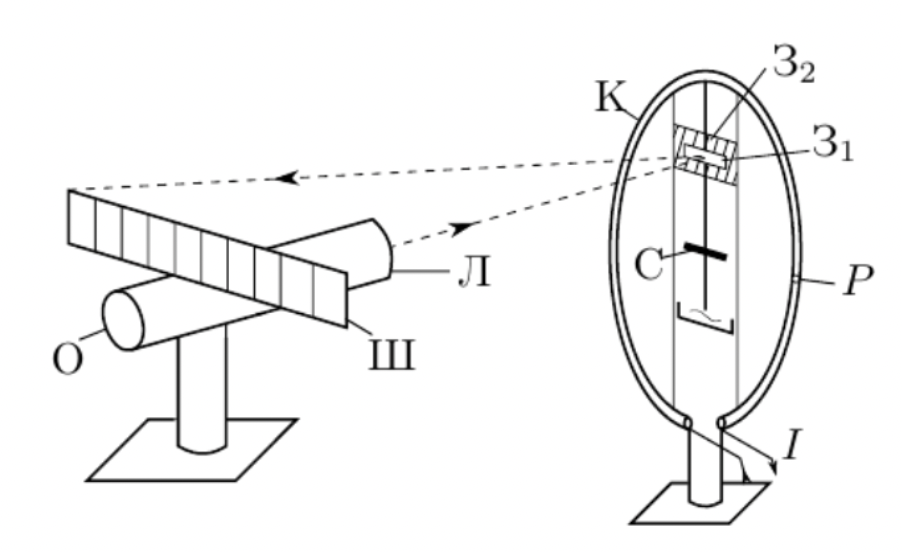
\includegraphics[width=6.5cm]{ustanovka.png}
    \caption{Схема экспериментальной установки.}
    \label{pic:2}
\end{wrapfigure}

\begin{figure}[h]
    \centering
    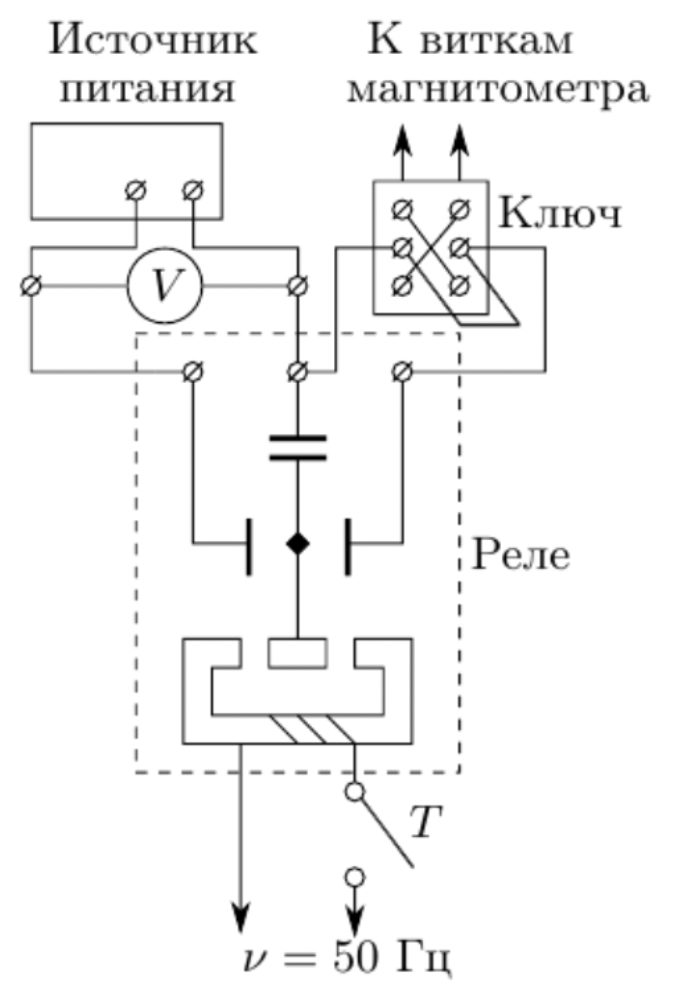
\includegraphics[width=0.5\textwidth]{circuit-scheme.png}
    \caption{Электрическая цепь, используемая в лабораторной.}
    \label{fig:circuit}
\end{figure}

\section{Ход работы:}
\subsection{Измерение горизонтальной составляющей магнитного поля Земли}
1) Настроим прибор, для этого включим осветитель и получим на экране 2 чётких световых "зайчика". Плавным поворотом кольца К вокруг вертикальной
оси совместим эти зайчики. Их четкость можно подрегулировать перемещением линзы Л вдоль оси осветителя. (Но это уже было настроено).


2) В отверстие P на горизонтальном диаметре кольца вставим намагниченный стержень и измерим смещение подвижного зайчика \(x_1\):
\[ x_1 = 5,5 см  \]

Поменяем ориентацию стержня и измерим отклонение зайчика:
\[ x_1 = 5,5 см \]
Отклонения  совпадают.

3) Измерим расстояние \(L\) от шкалы до зеркала:
\[ L = 81\; см \]


4) Измерим период малых колебаний стержня в магнитном поле Земли.
Для этого поставим стеклянный сосуд вблизи магнитометра и опустим на дно привязанный за середину намагниченный стержень. Плавным поворотом спицы, на которой закреплена нить, чуть приподнимим стержень и приближённо определим период малых крутильных колебаний:
\[ T = 7,3 с\]

5) Измерим параметры стержня, с помощью штангенциркуля:
\[ l = 4 см\]
\[ d = 0,5 cм\]
\[ m = 5,9 г\]

Радиус кольца (параметры установки):
\[ R = 20\; см \]

6) Рассчитаем величину горизонтальной составляющей магнитного поля Земли \(B_0\) по формуле:
\[ B_0 = \frac{2\pi}{TR}\sqrt{\frac{\mu_0JL}{2\pi Rx_1}} = 0.146\cdot10^{-4}\; T \]

Это значение, отличается от табличного \((B_0 = 5\cdot10^{-5}\; T)\). Они могут отличаться из-за помех от линий передач, географической локации и времени суток.

\subsection{Измерение электродинамической постоянной}

7) Уберем намагниченный стержень из гнезда магнитометра и собери
те электрическую схему, изображённую на \ref{fig:circuit}.

8) Убедимся, что зайчики совмещены в отсутствие тока через витки.

9) Включим в сеть источник питания и установите рабочее напряжение \( V = 100V \).

10) Замкнув ключ, подключим к цепи витки магнитометра.

11) Включив кнопкой К электровибратор, измерим напряжение на конденсаторе и отклонение \(x_2\) зайчика на шкале: \[ x_2 = 8см \]. Поменяв полярность с помощью ключа, повторим измерения: \[ x_2 = 8см \].

12) Запишем характеристики приборов и параметры установки:

\[ N = 44\]
\[ C = 1,09 мкФ\]
\[ \nu = 50 Гц\]

13) Рассчитайем токи по формулам:

\begin{enumerate}
    \item По формуле (СИ):
    \[ I_{СИ} = \frac{2B_0R}{\mu_oN}\tan{\phi_2} = 0.0052\; A \]  
    \item По формуле (СГС):
    \[ I_{СГС} = CV\nu = 16190805\; Био \]
\end{enumerate}

Можно вычислить значение электродинамической постоянной:
\[ c = \frac{1}{10}\frac{I_{CGS}}{I_{SI}} = 311361634\; м/с \]
Это значение почти совпадает с табличным \( (c = 29979245\; м/с)\).

\section{Выводы}
В ходе лабораторной работы была померена горизонтальная составляющая индукции магнитного поля Земли \( (B_0 = 0.146\cdot10^{-4}\; Tл) \). Это значение можно считаться достаточно точным, была экспериментально измерена электродинамическая постоянная \((c = 311361634\; м/с)\). Это значение довольно точно совпадает с табличным \( (c = 29979245\; м/с) \).

\end{document}